\section{Experimentación} 

\noindent En este momento contamos con varios algoritmos para resolver el problema de $k$-PMP:
\begin{enumerate}
  \item Algoritmo exacto.
  \item Algoritmo goloso.
  \item Heurísticas de búsqueda local y sus respectivas vecindades \textbf{(a)} swap y \textbf{(b)} jump.
  \item GRASP.
\end{enumerate}

El único de ellos que nos garantiza que la solución obtenida es óptima, exacta en este caso, es el algoritmo exacto.
El resto no exploran todo el espacio de soluciones sino que intentan recorrer un subconjunto acotado del mismo,
guiados por alguna heurística, y extraer la mejor del subconjunto explorado. El algoritmo exacto y el goloso
no requieren de configuración alguna. La búsqueda local y el GRASP sí requieren configuración y por lo tanto
dependiendo de la configuración que se utilice pueden devolver resultados diferentes para la misma instancia.
% recordar cuáles fueron las mejores configuraciones obtenidas para los configurables
Por esta razón, en sus respectivas secciones, nos dedicamos a analizar cuáles eran las mejores configuraciones.
Finalmente obtuvimos:

\begin{description}
  \item[búsqueda local] la vecindad \textit{jump} se mostró superior tanto en calidad como en tiempos de ejecución.
  \item[GRASP] profundidad de la elección de vértices 4 y profundidad de elección de conjuntos 4. 
\end{description}

% presentar el objetivo de la experimentación
El objetivo de la siguiente experimentación es comparar la performance de los algoritmos en función de la calidad de las soluciones obtenidas y de la performance en términos de tiempos de ejecución. Para ello
generamos un nuevo conjunto de instancias, diferente al conjunto con el cual fueron entrenadas, es decir
con el cual realizamos las experimentaciones para conseguir las mejores configuraciones. El conjunto de
instancias con el cual cada uno de los algoritmos fue entrenado no es necesariamente representativo, con
esto queremos decir que si bien obtuvimos una configuración superior en ese conjunto de instancias, esa
configuración no será necesariamente superior en otro conjunto de instancias o específicamente en 
familias particulares de grafos (instancias). Un claro ejemplo de esto es la familia de instancias
patológicas que describimos para el algoritmo goloso.
% aclarar cómo fue generado el nuevo conjunto de instancias
El conjunto de instancias fue generado de la misma manera que el que utilizamos para los tests de configuración
de GRASP. Al ser pseudoaleatorios con mínimas restricciones, como por ejemplo sobre la densidad mínima para que
las instancias no sean triviales, son independientes de dicho conjunto.

\subsection{Tiempos de ejecución}
% explicar que los tiempos del exacto sólo están hasta el 23 inclusive
En primer lugar, compararemos los tiempos de ejecución de los algoritmos tomando el promedio
sobre 100 instancias con una misma cantidad de vértices. El algoritmo exacto sólo
aparece graficado hasta $n=23$ porque para valores mayores toma demasiado tiempo.
% describir nuestras estimaciones
Nosotros estimamos que el exacto será el más lento por varios órdenes de magnitud y luego
vendrán GRASP, el goloso con la búsqueda local y luego el goloso. Creemos que será así
porque en cierta forma unos están incluidos en los otros. GRASP ejecuta un goloso aleatorizados
varias veces y a cada uno le aplica la heurística de búsqueda local, por lo cual en términos
de costos realiza el mismo trabajo que la heurística de búsqueda local pero muchas veces.
El goloso con la heurística de búqueda local primer ejecuta el goloso, por lo cual su costo
es el del goloso más el costo de la heurística de búsqueda local.

% gráficos
% explicar por qué creemos que es más ilustrativo presentar los mismos valores pero en distintos gráficos
\begin{figure}[H]
    \begin{minipage}[t]{\linewidth}
		\centering
		\frame{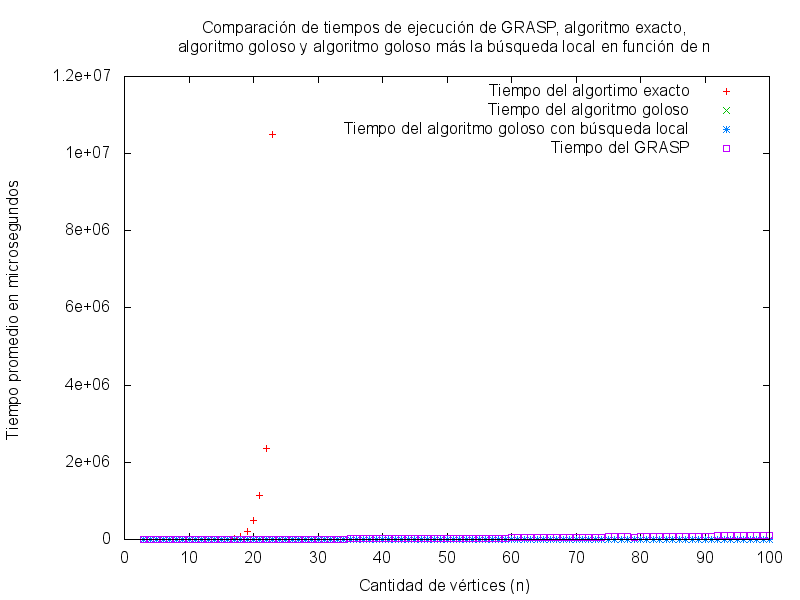
\includegraphics[width=\textwidth]{ejercicio-6-comparacion-tiempos.png}}
		\label{fig:ejercicio-6-comparacion-tiempos}
    \end{minipage}
\end{figure}
A partir de $n=19$ los tiempos del algoritmo exacto se vuelven muy grandes y se puede apreciar
que el crecimiento parece ser mucho mayor que exponencial. En comparación con los tiempos del exacto
el resto de los algoritmos parecen constantes, es por esto que decidimos graficar los mismos valores 
pero sin los tiempos del exacto para poder apreciar mejor sus diferencias y tendencias de crecimiento.
\begin{figure}[H]
    \begin{minipage}[t]{\linewidth}
		\centering
		\frame{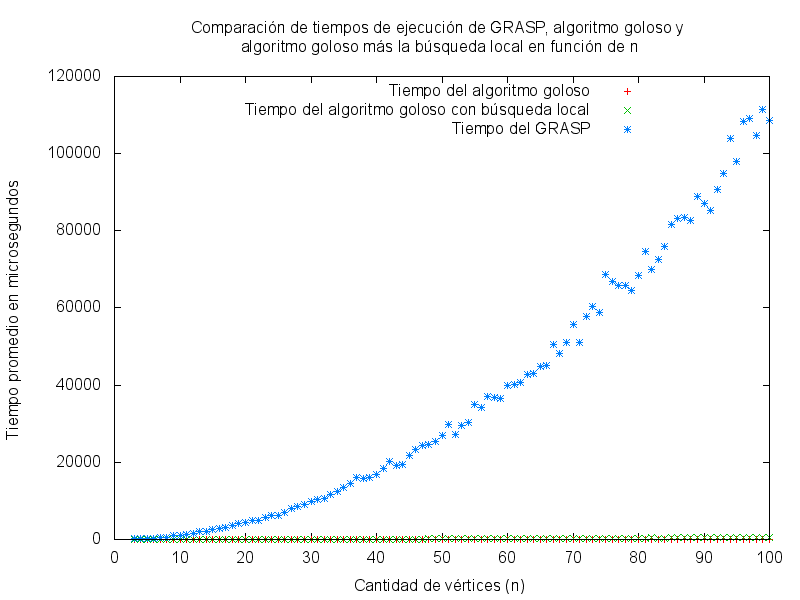
\includegraphics[width=\textwidth]{ejercicio-6-tiempos-menos-exacto.png}}
		\label{fig:ejercicio-6-comparacion-tiempos-menos-exacto}
    \end{minipage}
\end{figure}
Una vez más uno de los algoritmos tuvo tiempos de ejecución muy superiores al resto, en este caso fue GRASP.
Sin embargo, el crecimiento de GRASP se muestra mucho más suave que el presentado por el exacto en el gráfico anterior.
Como no se puede apreciar la diferencia entre el goloso con y sin búsqueda local decidimos graficarlos por separado
ya que comparándolos con GRASP parecen constantes.
\begin{figure}[H]
    \begin{minipage}[t]{\linewidth}
		\centering
		\frame{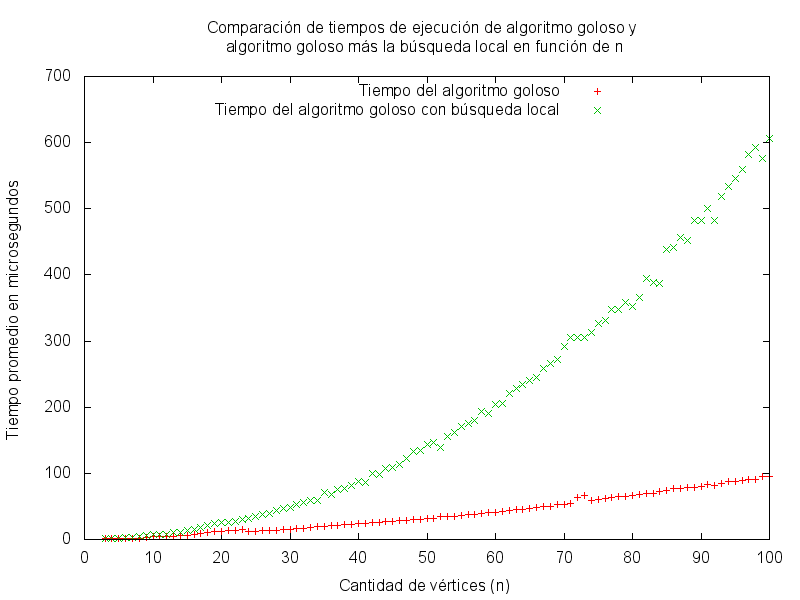
\includegraphics[width=\textwidth]{ejercicio-6-tiempos-menos-grasp.png}}
		\label{fig:ejercicio-6-comparacion-tiempos-menos-grasp}
    \end{minipage}
\end{figure}
Finalmente podemos apreciar la diferencia entre el goloso con y sin la búsqueda local. Vemos
que la búsqueda local no agrega sólo una constante al crecimiento del goloso, más bien aumenta 
su orden de magnitud ya que su crecimiento es claramente más veloz.
% análisis de los gráficos
El orden de méritos no presentó sorpresas pero los gráficos sí nos dejaron apreciar las diferencias entre 
uno y el siguiente. Podemos concluir que los tiempos de ejecución son órdenes de magnitud superiores entre
uno y otro algoritmo. El exacto presenta tiempos inutilizables en la práctica. GRASP tiene un performance
mucho mejor, la cual permite su utilización en la práctica, pero su costo es muy superior al del goloso con o sin búsqueda local.
Ahora necesitamos analizar la calidad de las soluciones que cada uno consigue para saber si el costo
temporal que implica GRASP redunda en una mejor calidad de sus soluciones o no.

\subsection{Calidad de las soluciones}
% describir nuestras estimaciones
Creemos que la calidad de las soluciones van a seguir el mismo orden que los tiempos de ejecución
principalmente por la inclusión de unos algoritmos en otros como ya explicamos en la sección anterior.
Creemos que la calidad de GRASP no va llegar a ser igual a la del exacto pero esperamos
que esté mucho más cerca que el goloso con y sin búsqueda local. Creemos que los dos mayores saltos
estarán entre el exacto y el GRASP y entre GRASP y los golosos.
% explicar que la calidad del exacto sólo está hasta el 23 inclusive
Decidimos primero graficar sólo con $n < 24$, los valores que alcanza el exacto, para poder apreciar
mejor las diferencias en este rango en el que contamos con la respuesta exacta.
% gráficos
\begin{figure}[H]
    \begin{minipage}[t]{\linewidth}
		\centering
		\frame{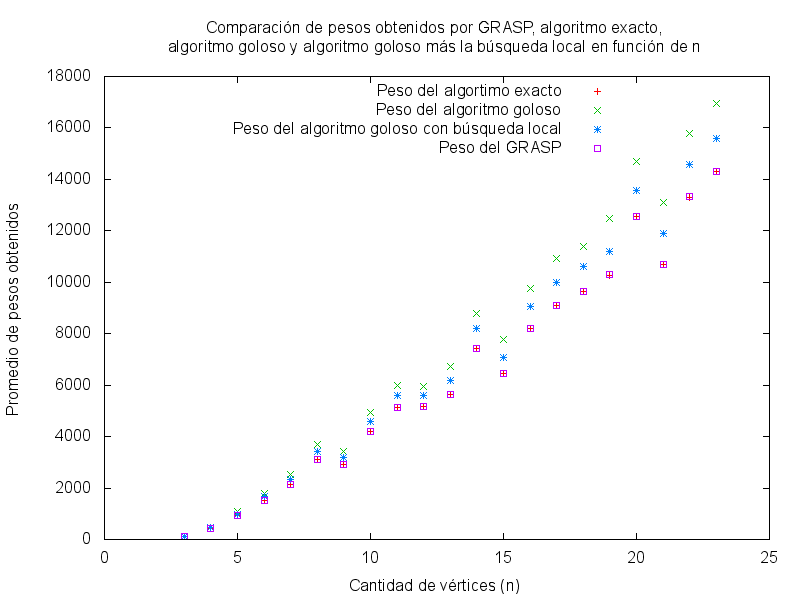
\includegraphics[width=\textwidth]{ejercicio-6-comparacion-calidad.png}}
		\label{fig:ejercicio-6-comparacion-calidad}
    \end{minipage}
\end{figure}

Sorprendentemente podemos ver que GRASP, al menos para éste rango de valores, tiene una calidad
igual que la del exacto. El orden es el que esperábamos pero no así la diferencia entre uno y el otro.
Sin embargo, parece que la tendencia es que la diferencia entre GRASP y goloso con búsqueda local y
goloso con búsqueda local y sin aumente junto con $n$.

\begin{figure}[H]
    \begin{minipage}[t]{\linewidth}
		\centering
		\frame{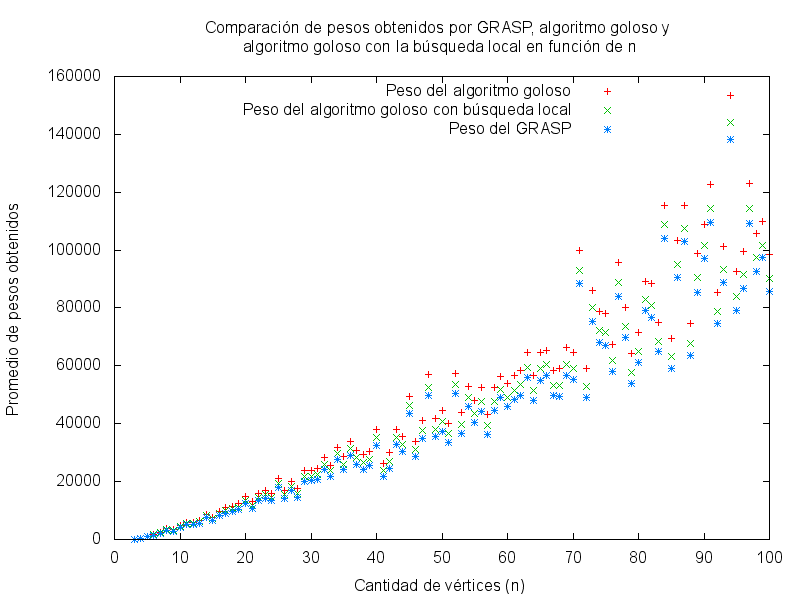
\includegraphics[width=\textwidth]{ejercicio-6-comparacion-calidad-sin-exacto.png}}
		\label{fig:ejercicio-6-comparacion-calidad-sin-exacto}
    \end{minipage}
\end{figure}

En este gráfico podemos ver que la diferencia entre GRASP y el goloso con búqueda local
parece no aumentar significativamente, si bien GRASP siempre consigue mejores resultados. La
diferencia entre goloso con búsqueda local y sin búsqueda local sí parece aumentar pero no queda
claro.
Finalmente decidimos graficar el error relativo presentado por todos los algoritmos con respecto al
exacto en el rango permitido. Este gráfico creemos que dará una idea más clara acerca de la distancia
entre la calidad de las soluciones de uno y otro algoritmo.

\begin{figure}[H]
    \begin{minipage}[t]{\linewidth}
		\centering
		\frame{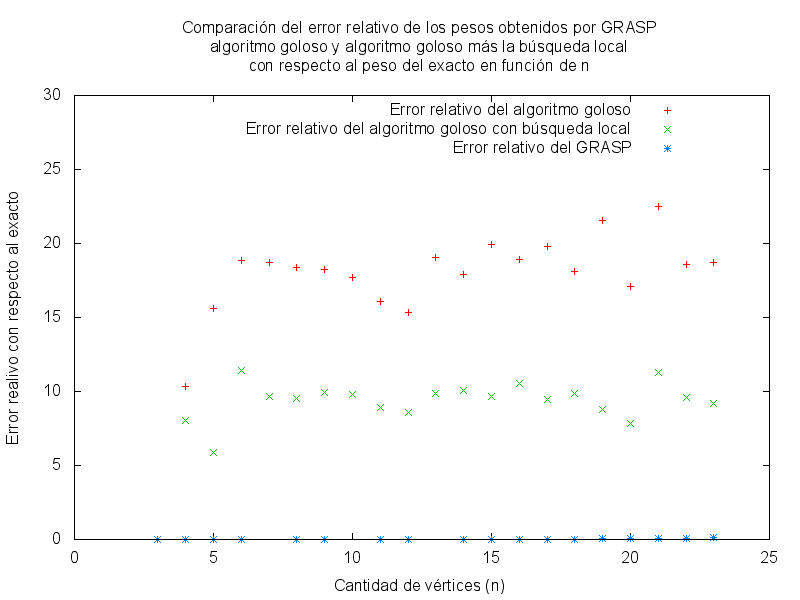
\includegraphics[width=\textwidth]{ejercicio-6-comparacion-calidad-error-relativo.png}}
		\label{fig:ejercicio-6-comparacion-calidad-error-relativo}
    \end{minipage}
\end{figure}

Se ve que el goloso con búsqueda local parece ubicarse generalmente apenas por debajo del $10\%$ y 
el goloso sin búsqueda local alrededor del $20\%$. La diferencia entre cada uno parece mostrar
un salto de aproximadamente $10\%$ de calidad entre uno y otro algoritmo. Si tuviéramos algún 
contexto particular éstas diferencias puede que cambien rotundamente.
% análisis de los gráficos

Pudimos ver que el costo temporal superior presentado por GRASP redunda en una mejor calidad, 
sin embargo, no queda claro que la ganancia sea muy grande, es decir parece que los tiempos
de ejecución son mucho mayores que la ganancia obtenida en la calidad de las soluciones. Ésto
claramente depende del contexto ya que ---por ejemplo--- el salto de $10\%$ que aproximamos de los
resultados obtenidos, en ciertos contextos puede ser una gran diferencia.


%\section{Conclusiones}
%
%Discutimos sobre criterios de parada y sobre la selección de candidatos de la golosa aleatorizada, y elegimos una configuración en base a los resultados obtenidos para un primer conjunto de instancias.
%
%Testeamos sobre dos criterios de parada y comentamos sus beneficios y problemas. En una aplicación real, sería conveniente por lo menos usar una combinación de ambos criterios, es decir, iteraciones sin mejora pero con un límite máximo de iteraciones global. Por otro lado, para distintos valores de $n$, vimos que es conveniente variar los límites para reducir el tiempo de ejecución, por lo cual sería interesante tener límites dinámicos según la cantidad de vértices del grafo de entrada.
%
%Para la selección de candidatos de la golosa aleatorizada, testeamos varios niveles de profundidad de elección de vértice y de elección de conjunto. No fue claro en particular que la mejor profundidad sea $(4,4)$, ya que aunque resultó ganadora, los errores relativos eran tan cercanos a cero que bien podría tratarse de una acumulación de los errores de cálculo inherentes a la aritmética finita. Sí es más claro que es más importante aleatorizar la elección del conjunto destino.
%
%Elegimos la configuración de iteraciones sin mejora y profundidad de elección de vértice-conjunto $(4,4)$ y comparamos los resultados del primer conjunto con un nuevo conjunto de iteraciones. Vimos que aunque los tiempos de ejecución se mantuvieron intactos, la calidad no fue la esperada, teniendo en algunos casos el doble de error relativo para el segundo conjunto. Esto sugiere que no hay garantía de que una configuración funcione relativamente bien siempre, la única garantía de calidad parece ser la cantidad de iteraciones que realiza la GRASP.
